\chapter{Problem Description} \label{ch_2:chapter}

In the present chapter the problem is presented, along with the proposal of new features to implement. It is structured as follows: Section \ref{ch_2:sect:aerostack} introduces the Aerostack framework, section \ref{ch_2:sect:requirements} presents the context of the problem and the requirements a replacement should have and section \ref{ch_2:sect:improvements} closes the chapter giving an overview on the improvements presented.

  \section{The Aerostack Framework} \label{ch_2:sect:aerostack}

    Aerostack is a software framework that helps developers design and build the control architecture of aerial robotic systems, integrating multiple heterogeneous computational solutions (i.e.: computer vision algorithms, motion controllers, self localization and mapping methods, planning algorithms, etc.).

    Aerostack is useful for building autonomous aerial systems in complex and dynamic environments and it is also a useful research tool for aerial robotics to test new algorithms and architectures.

    It was created to be available for communities of researchers and developers and it is currently an active open-source project. It provides some low level components as well as coordination processes and some planners. Figure \ref{ch_2:fig:aerostack_arqu} shows the general architecture of the framework. It is fully described in \cite{7502591} and \cite{Sanchez-Lopez2017} and publicly avaiable in \cite{aerostack_wiki_web}.

    \pagebreak
    \begin{figure}[ht]
      \centering
      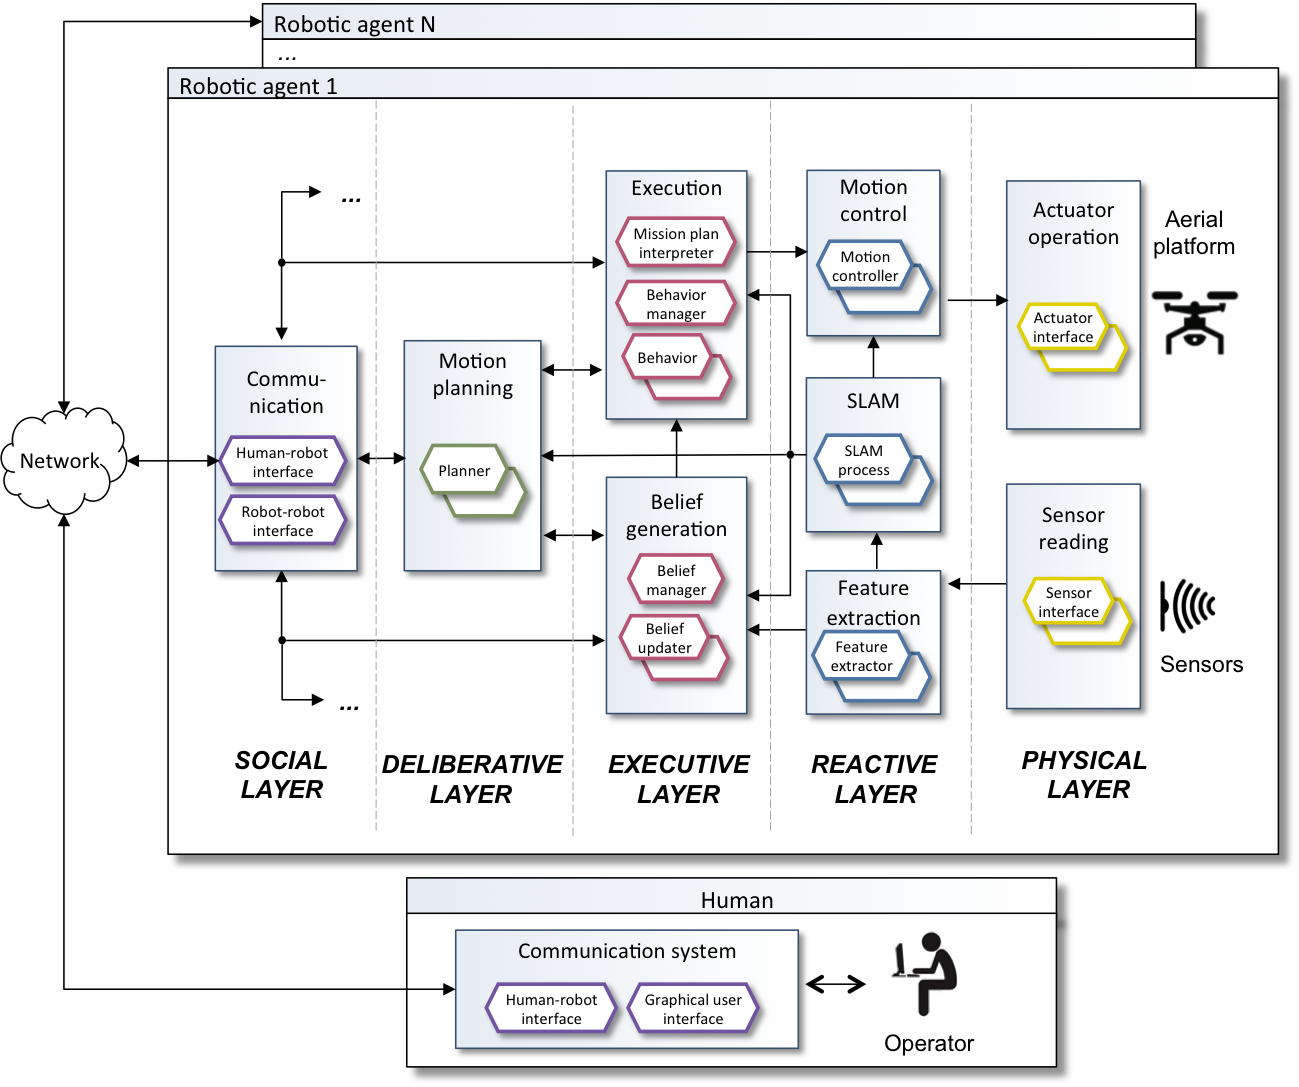
\includegraphics[width=0.8\textwidth]{AerostackArquitecture.png}
      \caption{The Aerostack architecture}
      \label{ch_2:fig:aerostack_arqu}
    \end{figure}

    This work will be specifically focused on the executive layer, the one pertaining the highest level of abstraction. The executive layer comprises the following components:

    \begin{itemize}
      \item Behavior coordinator: The process in charge of managing and monitoring the correct execution of behaviors, checks the necessary constraints and conditions to be met for a behavior to be executed. It is the central key to the whole behavioral system.
      \item Belief generation: This is the subsystem in charge of the store and retrieval of symbolic information, usually gathered from high level processors of sensory input, such as localization modules and behaviors.
    \end{itemize}

    When a behavior activation request arrives at the coordinator, it first checks the constraints of the requested behavior, if it conflicts with any other behavior, that behavior is deactivated. The next step is check the necessary processes, those are processes needed for the correct execution of the given behavior (more on this in the implementation chapter \ref{ch_4:chapter}). The coordinator activates those processes and then activates the behavior.

    This a flexible enough approach to specify pre and post conditions for a behavior to be executed, providing with the ability to check, at runtime, that the desired environment for a high level algorithm is ensured. This approach opens the door for programming and testing algorithms that enrich the capabilities of a robot in a robust and expressive manner.

  \section{Requirements} \label{ch_2:sect:requirements}

    As of the second version of Aerostack, the only localization techniques available are: visual localization based on the recognition of a special type of marker called Aruco (\cite{romeroramirez201838}) and odometry based localization. Aruco markers were first used for augmented reality applications, it is a fast and reliable technique to estimate the pose of the camera capturing the image. Although this system works fine for many applications, it imposes the need of preparing the environment, placing these markers in a very precise way and annotating it's exact position before the experiments. While this might not be a problem in an augmented reality like scenario, when it comes to live localization in unknown environment it becomes useless. Hence, a new system for localization is required.

    Along with the aforementioned localization technique comes the navigator which coordinates with a 2D geometric planner to accomplish the mission at hand. As the localization technique is to be changed, leading to a new way to perceive the environment, a new navigator and planner will also be necessary. 

  \section{Details of the New Features} \label{ch_2:sect:improvements}

    A lidar is going to be used as the main source for localization. The module in charge of this part is already present in the Aerostack framework, but it is not being used. Based on lidar input an occupancy grid is built. This occupancy grid is then used by the navigator, along with the planner instructions to build a motion plan to execute. Therefore, we will build:
    
    \begin{itemize}
      \item A module for localization and mapping based on lidar
      \item A module to do planning based on occupancy grids.
      \item A module capable of use the map and planning information to move the robot.
    \end{itemize}

    In the next chapter, the state of the arts algorithms chosen will be explained in depth.
